\documentclass[11pt]{article}
\usepackage{listings}
\usepackage{hyperref}
\usepackage{url}
\usepackage{tikz}
\usepackage{algorithm2e}
\usepackage{enumerate}
\usepackage{multicol}
\usepackage{alltt}
\usetikzlibrary{arrows,automata,shapes}
\tikzstyle{block} = [rectangle, draw, fill=blue!20, 
    text width=5em, text centered, rounded corners, minimum height=2em]
\tikzstyle{bt} = [rectangle, draw, fill=blue!20, 
    text width=1em, text centered, rounded corners, minimum height=2em]

\newtheorem{defn}{Definition}
\newtheorem{crit}{Criterion}

\newcommand{\handout}[5]{
  \noindent
  \begin{center}
  \framebox{
    \vbox{
      \hbox to 5.78in { {\bf Software Testing, Quality Assurance and Maintenance } \hfill #2 }
      \vspace{4mm}
      \hbox to 5.78in { {\Large \hfill #5  \hfill} }
      \vspace{2mm}
      \hbox to 5.78in { {\em #3 \hfill #4} }
    }
  }
  \end{center}
  \vspace*{4mm}
}

\newcommand{\lecture}[4]{\handout{#1}{#2}{#3}{#4}{Lecture #1}}
\topmargin 0pt
\advance \topmargin by -\headheight
\advance \topmargin by -\headsep
\textheight 8.9in
\oddsidemargin 0pt
\evensidemargin \oddsidemargin
\marginparwidth 0.5in
\textwidth 6.5in

\parindent 0in
\parskip 1.5ex
%\renewcommand{\baselinestretch}{1.25}

\begin{document}

\lecture{17 --- February 11, 2015}{Winter 2015}{Patrick Lam}{version 1}
We want to define du-pairs between callers and callees. Here's an example.

\begin{center}
\begin{multicols}{2}{
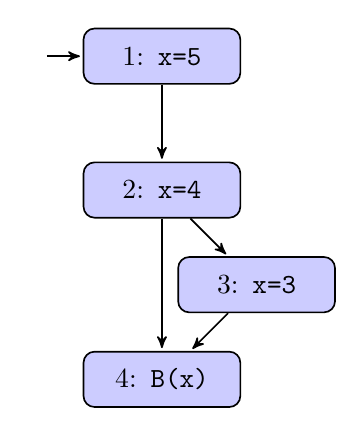
\begin{tikzpicture}[->,>=stealth',shorten >=1pt,auto,node distance=1.7cm,
                    semithick,initial text=]
  \node[initial,block]   (1)                     {1: \tt x=5};
  \node[block]           (2) [below of=1] {2: \tt x=4};
  \node[block]           (3) [below right of=2] {3: \tt x=3};
  \node[block]           (4) [below left of=3] {4: \tt B(x)};

  \path (1) edge node {} (2)
        (2) edge node {} (3)
            edge node {} (4)
        (3) edge node {} (4);
\end{tikzpicture}
}{
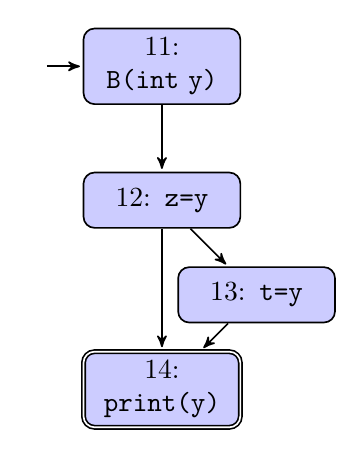
\begin{tikzpicture}[->,>=stealth',shorten >=1pt,auto,node distance=1.7cm,
                    semithick,initial text=]
  \node[initial,block]   (1)                     {11: \tt B(int y)};
  \node[block]           (2) [below of=1] {12: \tt z=y};
  \node[block]           (3) [below right of=2] {13: \tt t=y};
  \node[block,accepting] (4) [below left of=3] {14: \tt print(y)};

  \path (1) edge node {} (2)
        (2) edge node {} (4)
            edge node {} (3)
        (3) edge node {} (4);
\end{tikzpicture}
}
\end{multicols}
\end{center}
We'll say that the \emph{last-defs} are 2, 3; the \emph{first-use}
is 12. We formally define these notions:
\begin{defn}
\emph{(Last-def)}. The set of nodes $N$ that define a variable {\tt x}
for which there is a def-clear path from a node $n \in N$ through a call 
to a use in the other unit.
\end{defn}
\begin{defn}
\emph{(First-use)}. The set of nodes $N$ that have uses of {\tt y} and
for which there exists a path that is def-clear and use-clear
from the entry point (if the use is in the callee) or the callsite
(if the use is in the caller) to the nodes $N$.
\end{defn}

We need the following side definition, analogous to that of def-clear:
\begin{defn} A path $p = [n_1, \ldots, n_j]$ is \emph{use-clear} with
respect to $v$ if for every $n_k \in p$, where $k \neq 1$ and $k \neq j$,
then $v$ is not in $\mbox{use}(n_k)$.
\end{defn}

In other words, the last-def is the definition that goes through the call
or return, and the first-use picks up that definition.

\newpage
Here are two more examples:
\begin{multicols}{2}{
\begin{verbatim}
  x = 14;   // last-def
  y = g(x);
  print(y); // first-use

  int g(a) {
    print(a); // first-use
    b = 24;   // last-def
    return b;
  }



  
\end{verbatim}
}{
\begin{verbatim}
main() {
  x = 1;
  x = 2; // last-def
  if (...) { x = 3; /* last-def */ }
  B(x);
}
B(int y) {
  if (...) {
    Z = y; // first-use
  } else {
    T = y; // first-use
  }
  print(y);
}
\end{verbatim}
}
\end{multicols}

One can create pairs of triples linking last-defs and first-uses;
characterize a last-def or a first-use by the method name, the
variable name, and the statement, and then link them.

Tests can, of course, go beyond just testing the first-use.
Our first-use and last-def definitions, however, make testing
slightly more tractable. We could, of course, carry out full
inter-procedural data-flow, i.e. covering all du-pairs,
but this would be more expensive.

\section*{Syntax-Based Testing}
We are going to completely switch gears now. We will see two applications of context-free grammars:
\begin{enumerate}
\item input-space grammars: create inputs (both valid and invalid)
\item program-based grammars: modify programs (mutation testing)
\end{enumerate}


\paragraph{Mutation testing.} The basic idea behind mutation testing is to improve your test suites
by creating modified programs (\emph{mutants}) which force your test suites
to include test cases which verify certain specific behaviours of the
original programs by killing the mutants.

\subsection*{Generating Inputs: Regular Expressions and Grammars}

Consider the following Perl regular expression for Visa numbers:

\begin{verbatim}
                        ^4[0-9]{12}(?:[0-9]{3})?$
\end{verbatim}
%(This regexp is different from the syntax you saw in automata/compilers
%classes, but could be expressed in the standard way too, as it has no
%backrefs.)

Idea: generate ``valid'' tests from regexps and invalid tests by 
mutating the grammar/regexp. {\sf (Why did I put valid in quotes? What
is the fundamental limitation of regexps?)}
\\[4em]

%Fundamental limitation of regexps: \\[2em]
% can't count, e.g. can't balance parens.

Instead, we can use grammars to generate inputs (including sequences
of input events).

Typical grammar fragment:

\begin{eqnarray*}
\mbox{mult\_exp} &=& \mbox{unary\_exp} \mid \mbox{mult\_exp {\tt STAR} unary\_arith\_exp} \mid \mbox{mult\_exp {\tt DIV} unary\_arith\_exp}; \\
\mbox{unary\_exp} &=& \mbox{quant\_exp} \mid \mbox{unary\_exp {\tt DOT INT}}
\mid \mbox{unary\_exp up};\\
&\vdots& \\
\mbox{start} &=& \mbox{header}^? \mbox{declaration}^*
\end{eqnarray*}

\paragraph{Using Grammars.} Two ways you can use input grammars for
software testing and maintenance:
\begin{itemize}
\item recognizer: can include them in a program to validate inputs;
\item generator: can create program inputs for testing.
\end{itemize}
Generators start with the start production and replace nonterminals
with their right-hand sides to get (eventually) strings belonging to 
the input languages.

We specify three coverage criteria for inputs with respect to a grammar $G$.
\begin{crit}
{\bf Terminal Symbol Coverage} (TSC). TR contains each terminal of grammar $G$.
\end{crit}
\begin{crit}
{\bf Production Coverage} (PDC). TR contains each production of grammar $G$.
\end{crit}
\begin{crit}
{\bf Derivation Coverage} (DC). TR contains every possible string derivable
from $G$.
\end{crit}
PDC subsumes TSC. DC often generates infinite test sets, and even if
you limit to fixed-length strings, you still have huge numbers of inputs.


\paragraph{Another Grammar.}~\\

{\sf 
\begin{tabular}{lcl}
roll &=& action$^*$ \\
action &=& dep $\mid$ deb \\
dep &=& {\tt "deposit"} account amount \\
deb &=& {\tt "debit"} account amount \\
account &=& digit \{ 3 \} \\
amount &=& {\tt "\$"} digit$^+$ {\tt "."} digit \{ 2 \} \\
digit &=& ["0" -- "9"]
\end{tabular}
}

\paragraph{Examples of valid strings.}~\\[4em]
%\begin{verbatim} 
% deposit 739 $12.35
% deposit 929 $33.20
% debit 739 $6.00
%\end{verbatim}

Note: creating a grammar for a system that doesn't have one, but should,
is a useful QA exercise. Using this grammar at runtime to validate inputs
can improve software reliability, although it makes tests generated
from the grammar less useful.


\paragraph{Some Grammar Mutation Operators.} 
\begin{itemize}
\item Nonterminal Replacement; e.g. \\
{\sf dep = {\tt "deposit"} account amount $\Longrightarrow$
 dep = {\tt "deposit"} amount amount}\\[4em]
(Use your judgement to replace nonterminals with similar nonterminals.)

\item Terminal Replacement; e.g. \\
{\sf amount = {\tt "\$"} digit$^+$ {\tt "."} digit \{ 2 \} 
$\Longrightarrow$ amount = {\tt "\$"} digit$^+$ {\tt "\$"} digit \{ 2 \} } \\[4em]

\item Terminal and Nonterminal Deletion; e.g.\\
{\sf dep = {\tt "deposit"} account amount $\Longrightarrow$
 dep = {\tt "deposit"} amount}\\[4em]

\item Terminal and Nonterminal Duplication; e.g.\\
{\sf dep = {\tt "deposit"} account amount $\Longrightarrow$
 dep = {\tt "deposit"} account account amount}\\[4em]
\end{itemize}

\paragraph{Using grammar mutation operators.}
\begin{enumerate}
\item mutate grammar, generate (invalid) inputs; or,
\item use correct grammar, but mis-derive a rule once---gives ``closer''
inputs (since you only miss once.)
\end{enumerate}

\paragraph{Why test invalid inputs?} Bill Sempf (@sempf), on Twitter: ``QA Engineer walks into a bar. Orders a beer. Orders 0 beers. Orders 999999999 beers. Orders a lizard. Orders -1 beers. Orders a sfdeljknesv.''

If you're lucky, your program accepts strings (or events) described by a regexp or a grammar. But you might not use a parser or regexp engine. Generating using the regexp or grammar helps detect deviations, both right now and in the future.

As you saw in Assignment 1, it's the easiest thing to overlook invalid inputs. Yet they may lead to undefined behaviour.

What we'll do is to mutate the grammars and generate test strings from the mutated grammars.

Some notes:
\begin{itemize}
\item Book claims we don't have much experience using grammar-based operators.
\item Can generate strings still in the grammar even after mutation.
\item Recall that we aren't talking about semantic checks.
\item Some programs accept only a subset of a specified larger language,
e.g. Blogger HTML comments. Then testing intersection is useful.
\end{itemize}



\end{document}
